\documentclass[12pt,english]{article}

\usepackage{amsmath,amsfonts,amssymb,amscd,amsthm,amsbsy,alltt,bera,upref,fancyvrb}
\usepackage[T1]{fontenc}
\usepackage{babel}
\usepackage{graphicx}

\textheight=8.5truein
\textwidth=6.0truein
\hoffset=-.5truein
\voffset=-.5truein
\pagestyle{headings}
\footskip=36pt
\swapnumbers
\DefineVerbatimEnvironment{code}{Verbatim}{fontsize=\small}
\DefineVerbatimEnvironment{example}{Verbatim}{fontsize=\small}


\makeatletter
\def\and{%
  \end{tabular}%
  \hskip 1em \@plus.10fil\relax
  \begin{tabular}[t]{c}}
\makeatother
\makeindex


\title{Technical Report: The Austinites}
\author{
  Sheeyla Garcia\\
  \and
  Jesus Hernandez\\
  \and
  Kyle Nicola\\
  \and
  Stephen Ridings\\
  \and
  Carlos Rodriguez\\
  \and
  Mark Sandan\\  
}
\date{ }
\begin{document}
\thispagestyle{plain}
\maketitle
 
 [splash page]
 
\tableofcontents

\section{Introduction} 
The website we are designing is about the 2014 Austin City Limits (ACL) music festival. The website design has three main pages: Artists, Stages, and Sponsors.
The website allows anyone to view pages about current Artists, Sponsors, and Stages. The technologies used are PythonAnywhere, Python 3.4, Django 1.6,
Twitter Bootstrap 3.2, Apiary, and the database sqlite3. PythonAnywhere is used to host the site using the Django web-framework to 
construct the necessary models and views to handle HTTP requests. Twitter Bootstrap is used to organize common data among different
types of pages into a base template HTML file. 

The database we chose to test with (see Tests) is sqlite3. We currently don't use it to load any data to render the HTML pages.

\section{Design}
Our current design of the website uses HTML and Twitter Bootstrap to stylize each page and PythonAnywhere to host the page. 
Using Django's templating language we are able to reuse html files by extending from them. Currently we only have a single base html page that
uses Twitter Bootstrap. We have nine pages in static HTML that provide examples of the web page design and content.

[UML model here]
\begin{figure}[h]
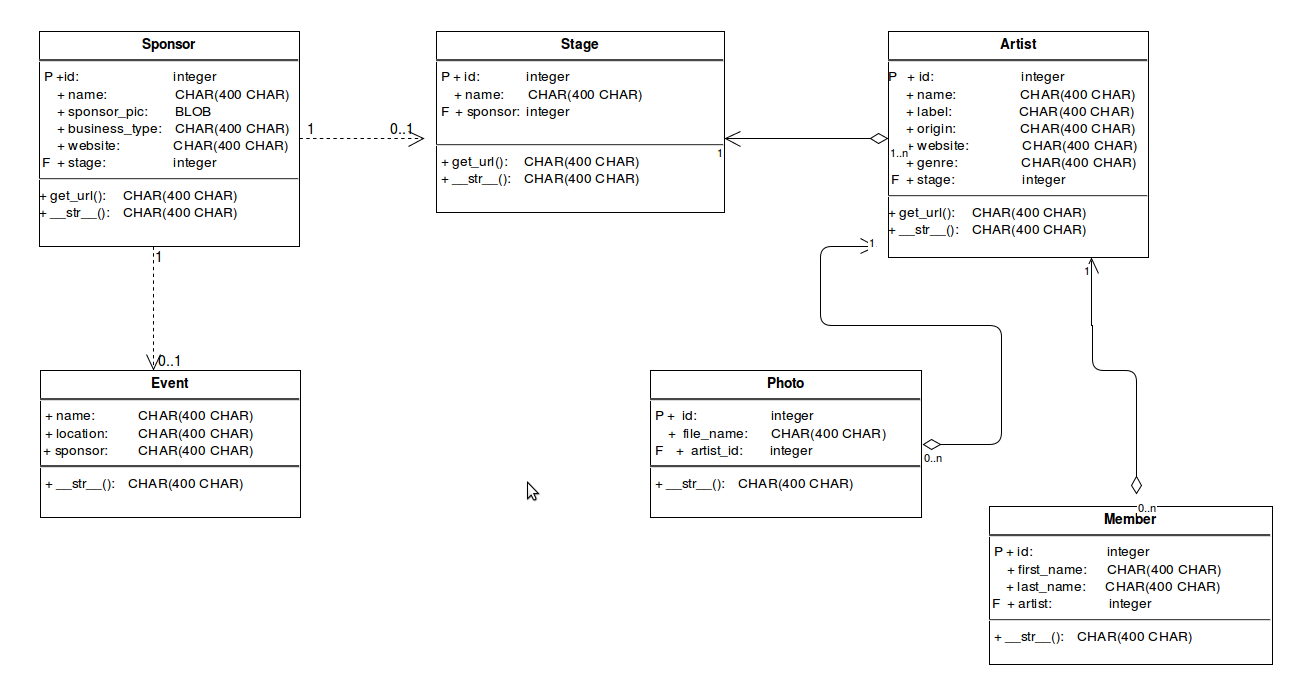
\includegraphics[width=\textwidth]{UML}
\end{figure}

\subsection{App Design}
The current directory structure on PythonAnywhere is outlined below for reference to files:

[tree -d layout here]

\subsection{Web Pages}
Each web page has basic information about a particular artist, sponsor, or stage involved in the ACL music festival.
Each page includes a bio, video, official website, Youtube channel, a Twitter feed, and Picture.
\subsubsection{Artists}
Artist Pages can be reached from the home page or from Stage pages depending on whether the Artist played on
a Stage that was hosted by a Sponsor. 
\subsubsection{Sponsors}
Sponsor pages can be reached from the home page or from 

\subsubsection{Stages}


[Example Relation scheme here]

\subsection{RESTful  API}
The REST API for the website currently documents only GET 

\subsection{Django Models}
The Django models created represent the entities we intend to keep in the database for the future when use dynamically loaded pages.
The following subsections document the attributes and intended functionality of each class instance method.
\subsubsection{Artist}

\subsubsection{Sponsor}

\subsubsection{Stage}

\subsubsection{Photo}
The Photo class extends from the Django models.Models class and has two main attributes: 
\begin{verbatim}
file_name
artist
 \end{verbatim}

The Foreign key is the artist that the Photo is associated with. Thus the Artist is a parent
of a one-to-many relationship with a Photo. Currently the only method defined is 
\begin{verbatim}
__str__ 
\end{verbatim} 

\subsubsection{Event}

\subsubsection{Member}

Detailed documentation of each of our Django models
\section{Tests}



\end{document}
